\documentclass[twocolumn]{article}

\usepackage{graphicx}
\usepackage{url}
\usepackage[margin=0.75in]{geometry}
\usepackage{titlesec}
\usepackage{booktabs}
\usepackage{tabularx}
\usepackage{xcolor}
\newcommand{\authorinput}[1]{\par\smallskip\noindent\begin{minipage}{\linewidth}\textcolor{red!65!black}{\textbf{Author input:} #1}\end{minipage}\par\smallskip}

\raggedbottom
\titlespacing*{\section}{0pt}{1.5ex}{0.5ex}

\title{Beyond Tool Calling: Domain-Specific Workspaces
for Personalized AI Agents}
\author{Wei-Lin Chou}
\date{}

\begin{document}


\maketitle








\section*{Abstract}
\noindent

Personal AI agents can use external tools to execute complex tasks, but managing workflows that span multiple services and sessions introduces challenges in maintaining task state, coordinating actions, and incorporating user preferences. General-purpose browser automation and tool interfaces provide access to external systems, but the extent to which dedicated software environments improve agent performance remains unclear.

This paper presents Lookout, an agent-native workspace designed to support personal AI agents in managing job search workflows. Lookout provides structured access to job opportunities, persistent application records, and tools for executing and tracking actions on behalf of users. The system separates agent reasoning and personalization from domain-specific workflow management, allowing existing personal agents to operate through a shared software environment. Typed operations, selectively retrieved context, and persistent workflow records allow the workspace to preserve changing job-search information across agent sessions.

We formulate an evaluation to test whether providing agents with this workspace improves task completion, execution efficiency, and workflow continuity compared with agents using general-purpose tools. We implement controlled JOB and COM task families and a Langfuse reporting pipeline that separates quality, execution time, user effort, and cost. This draft describes the system and evaluation protocol; experimental results and conclusions remain to be added.

\section{Introduction}
\subsection{Motivation}
Job searching combines repeated execution with decisions requiring personal judgment. An agent can find roles and prepare materials, but must also preserve preferences, incorporate corrections, distinguish draft work from completed actions, and resume after user input. These responsibilities span sessions and services. A submission attempt with an unknown outcome, for example, requires verification before another attempt; a fluent progress message cannot resolve the uncertainty.

Personal agents already offer tools, memory, and scheduled tasks. The question is what a shared domain workspace adds. Lookout gives agents persistent application records and gives users a direct interface for inspecting and correcting them. This paper studies whether that shared state and validated action interface improve execution relative to a general-purpose agent with persistent files. The comparison must account for the workspace's additional discovery, retrieval, and verification costs.

\subsection{Research Question and Contributions}
This paper investigates whether dedicated software environments improve how personal AI agents manage ongoing tasks on behalf of users. Specifically, we examine whether an agent-native workspace offers measurable advantages over configuring equivalent workflows directly through an agent's tools, memory, and scheduled automations. We focus on three aspects of performance: task completion, execution efficiency, and the amount of human supervision required.

To study this question, we developed Lookout, a job-search workspace that allows existing personal agents to discover opportunities, manage applications, and coordinate actions with users through structured tools and persistent workflow records.

The primary contributions of this work are:

Agent-native workspace architecture: A design that combines typed domain operations, selectively loaded context, and persistent workflow state to coordinate delegated execution and human oversight.

System implementation: Lookout, an MCP-accessible job-search workspace integrating opportunity discovery, application management, and user review workflows.

Evaluation infrastructure: Versioned JOB and COM scenarios, independent artifact-based grading, and structural Langfuse exports for comparing workspace-supported agents with a persistent-file baseline. A repeated measured campaign remains planned.
\section{Background and Related Work}
\subsection{Long-Horizon Agent Execution}

Long-horizon workflows require agents to coordinate dependent actions, maintain task constraints, and respond to changes throughout execution. Yuan et al.~\cite{osworld} introduced OSWorld 2.0, a benchmark containing 108 realistic computer-use workflows that take human users a median of approximately 1.6 hours to complete. Their evaluation identified recurring failures in tracking constraints, responding to newly available information, and verifying completed actions. In the cited paper, the strongest evaluated configuration achieved a 20.6\% full-task completion rate under a 500-step budget, demonstrating the difficulty of sustained execution even for capable agents.

These findings are relevant to job search workflows, where agents must manage multiple applications with different requirements and changing statuses. However, OSWorld 2.0 primarily evaluates execution within individual workflows rather than the coordination of ongoing responsibilities across sessions.

\subsection{Persistent State Management}
One approach to improving long-horizon reliability is to maintain an explicit representation of task progress outside the agent's conversational history. Zou et al.~\cite{stateharness} proposed StateHarness, a runtime framework that records project decisions, relevant findings, dependencies, and unresolved work for coding agents. On RefactorBench, StateHarness improved full-chain task completion from 29.4\% to 35.3\%, suggesting that structured state management can improve execution consistency.

Ding et al.~\cite{alwayson} examined this problem more broadly in their survey of always-on agents. They characterize persistent agents as systems that maintain not only memory, but also task records, permissions, commitments, and externally executed actions. Their analysis highlights the importance of governing and recovering operational state as agents continue working over time.

These studies motivate explicit persistent state, although StateHarness focuses on software development and the survey does not directly evaluate domain-specific applications shared between agents and users.

\subsection{Human-Agent Collaboration}
Long-running tasks also require coordination between automated execution and human judgment. Hayati et al.~\cite{kolab} introduced Kolab, a benchmark based on over 115 hours of interactions between 50 professionals and AI agents. Their findings show that evaluating autonomous task completion alone does not adequately capture collaboration quality. Agents must also account for how users adopt, revise, or reject their contributions throughout a workflow.

This distinction is relevant to job searching, where an agent may independently discover opportunities and prepare materials while requiring user input before consequential actions. Managing these interactions introduces requirements beyond task execution, including presenting pending decisions, incorporating feedback, and resuming work afterward.

\subsection{Executable Agent Benchmarks}
SWE-bench evaluates repository repairs through executable tests, including checks that previously working behavior remains intact~\cite{swebench}. MLE-bench packages ML-engineering tasks with local grading and specifies the model, scaffold, resources, and runtime needed to interpret scores~\cite{mlebench}. We use these as methodological references: freeze the starting environment, score observable artifacts, and test preservation alongside progress. Our job-search cases use fictional event streams and domain-state checks; they are neither SWE-bench tasks nor MLE-bench scores. SWE-agent's interface ablations further motivate testing the cost and benefit of domain tools separately from the underlying model~\cite{sweagent}.

\section{Problem Formulation}
\subsection{Problem Definition}
A personal agent manages interdependent tasks whose context, progress, and authorization can change across sessions. In job search, discovery feeds preparation; missing facts require user input; later employer events change the next action. Execution must preserve prior decisions, avoid conflicting actions, and resume after corrections. We ask whether a shared domain workspace supports these responsibilities more effectively than the agent's general-purpose tools and persistent files.

\subsection{Workspace Requirements}
We identify three requirements for supporting long-running workflows delegated to personal AI agents:

State continuity: Preserve task progress, prior decisions, and execution outcomes across sessions to support reliable resumption without duplicating completed work.

Controlled execution: Enforce authorization constraints and workflow transitions, including safeguards against repeated actions when execution outcomes are uncertain.

Human-agent coordination: Allow users to inspect ongoing work, review consequential decisions, and provide feedback that agents can incorporate into subsequent execution.

\begin{figure*}[t]
    \centering
    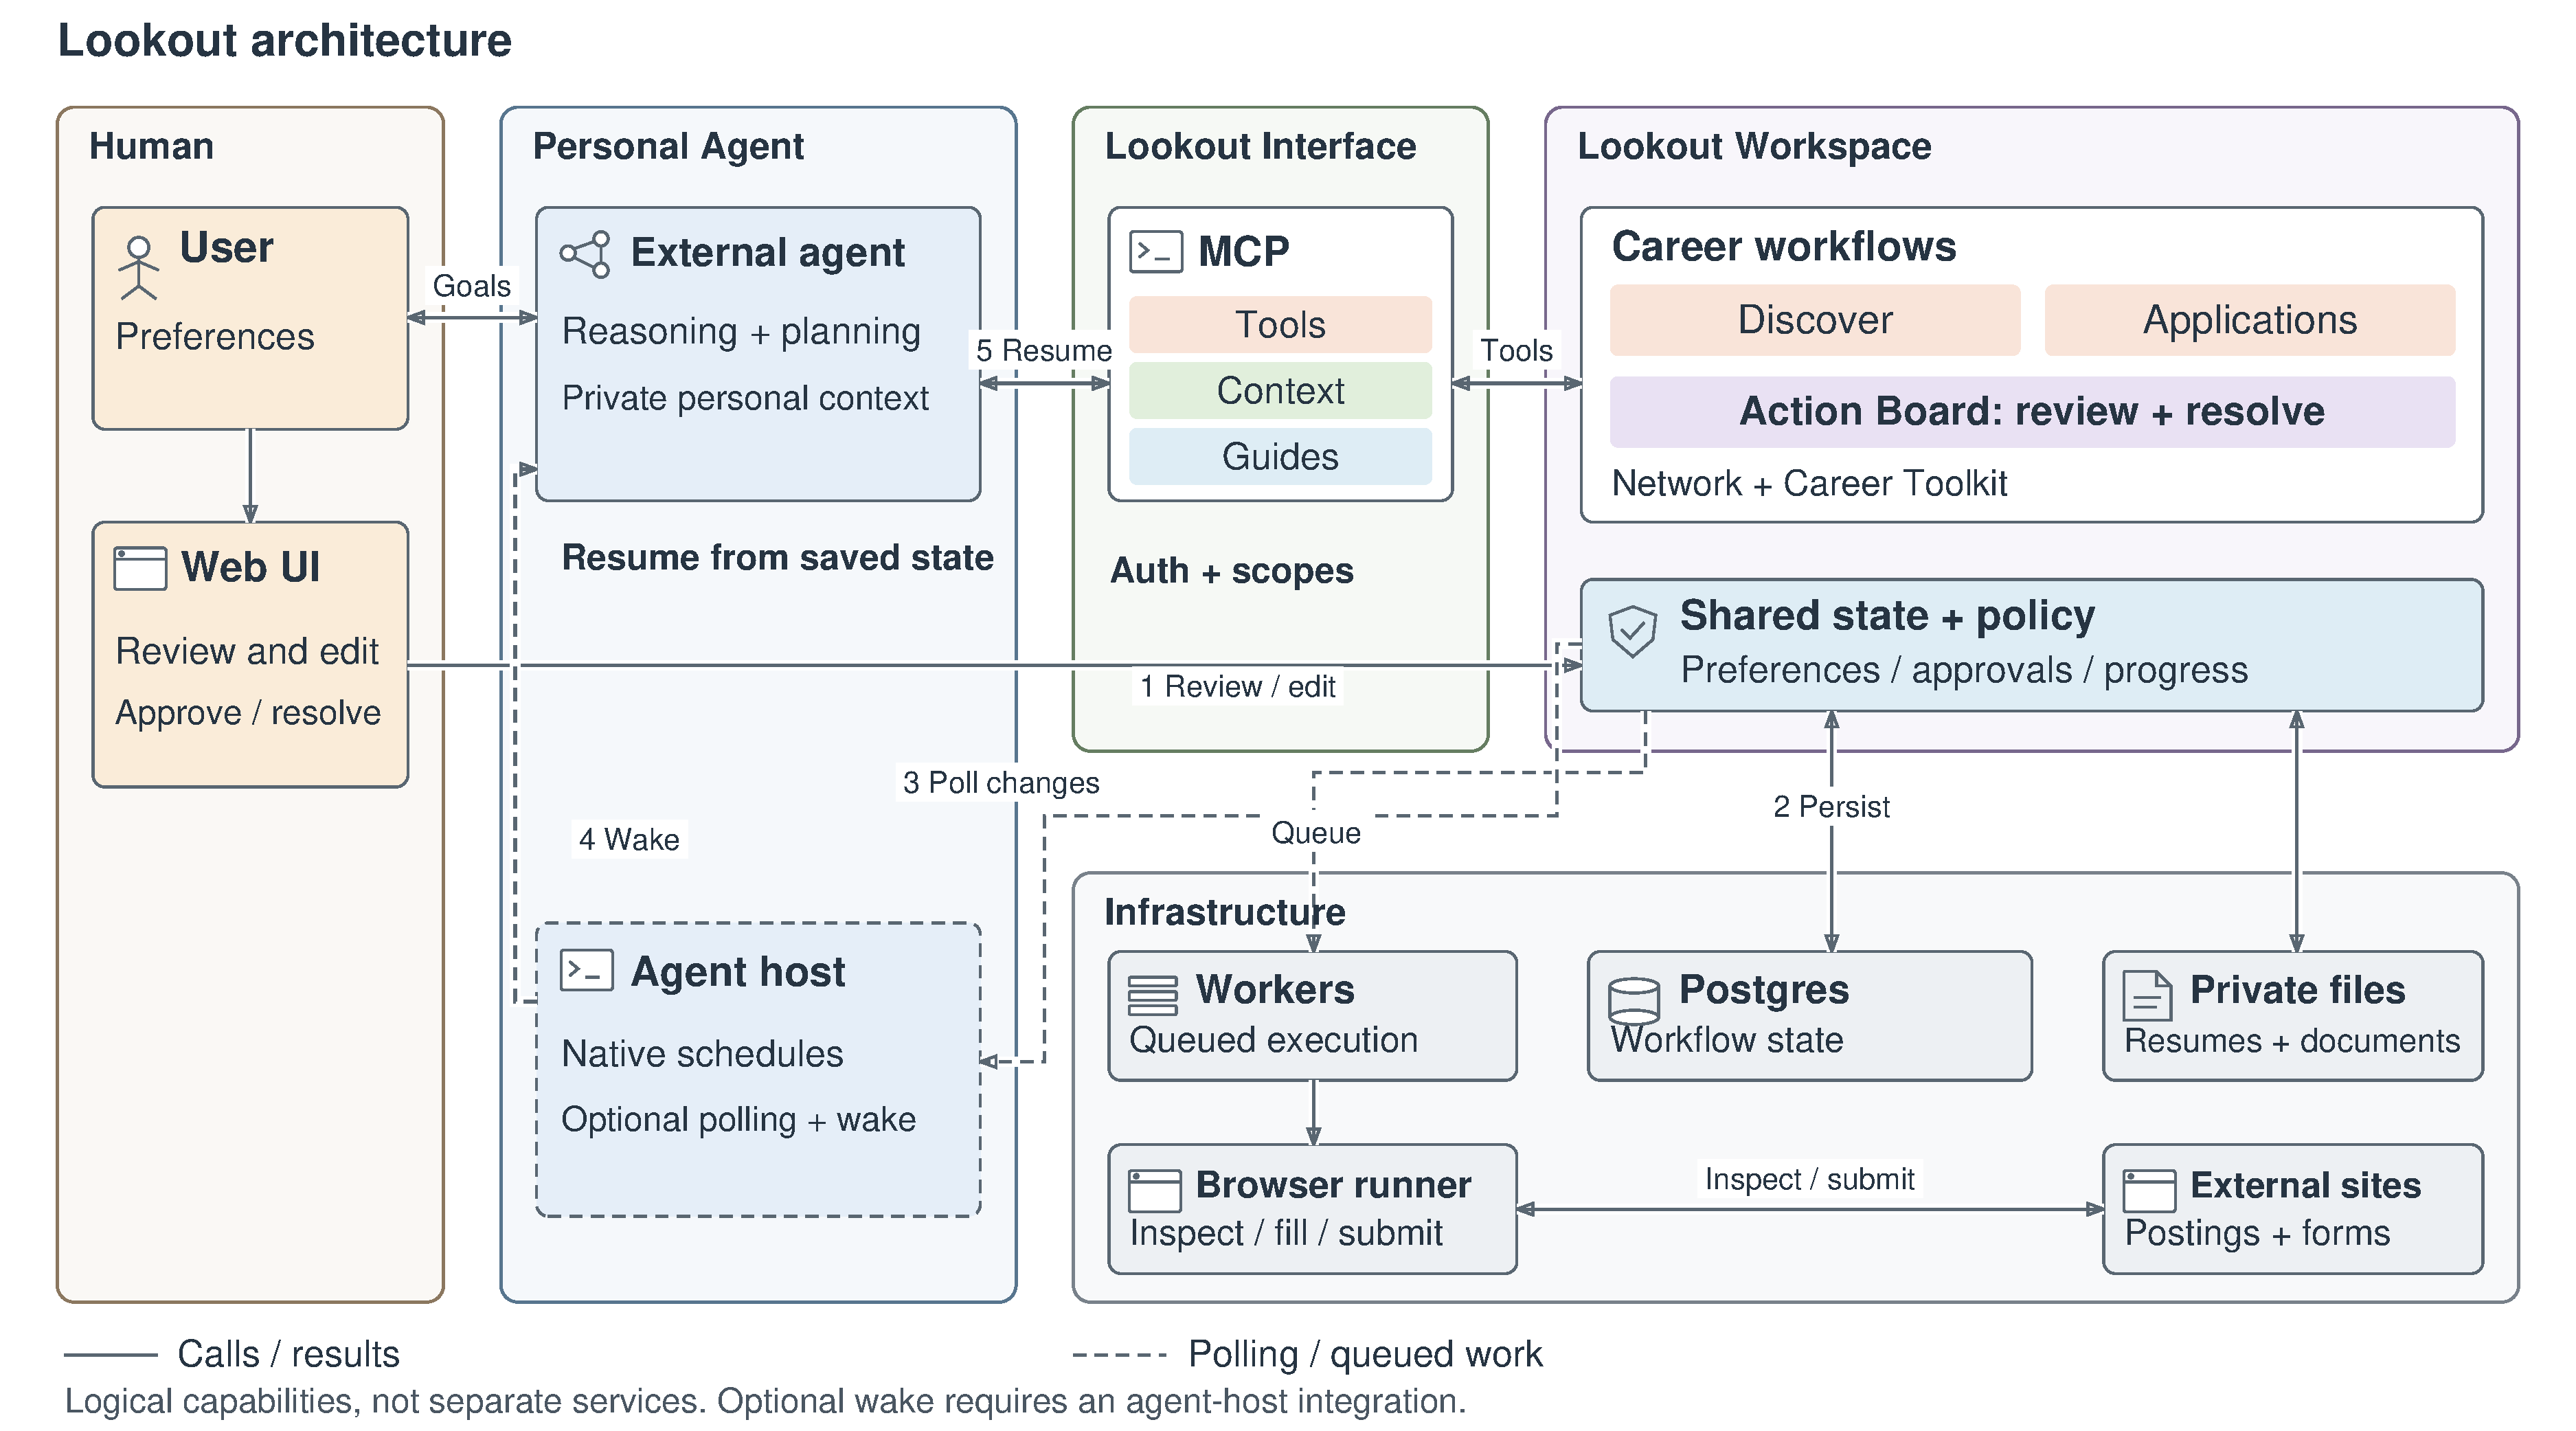
\includegraphics[width=0.95\textwidth]{docs/figures/lookout-architecture.pdf}
    \caption{Lookout system architecture showing
    the interactions between users, personal agents,
    MCP interfaces, and workspace services. The figure summarizes logical boundaries; its workers/browser path includes retained deterministic application code that is currently paused. Current AI Apply requests use the external agent host for browser execution.}
    \label{fig:architecture}
\end{figure*}


\section{System Design}


\subsection{Architecture Overview}

Lookout separates personal-agent reasoning from domain-specific workflow management. As illustrated in Figure~\ref{fig:architecture}, the architecture consists of an external personal agent, an authenticated Model Context Protocol (MCP) interface, persistent workspace services, a user-facing interface, and execution infrastructure.

The external agent is responsible for reasoning, planning, and applying knowledge of the user to job-search activities. Lookout provides the environment through which those activities are organized and executed. Its backend supports opportunity discovery, application management, networking records, career preparation, and workflow coordination. A shared persistence layer maintains application progress and user decisions independently of individual agent sessions.

The system exposes two interfaces to the same underlying workspace. Agents interact through MCP tools, while users inspect and modify records through the web interface. This separation allows either participant to update ongoing work without requiring the other to remain continuously active.

\subsection{Tool Feedback and Context Retrieval}
SWE-agent treats the available actions and returned observations as an interface that can be designed for an agent~\cite{sweagent}. Lookout applies this principle to job-search records: MCP operations expose domain actions with JSON schemas, ownership checks, and expected revisions. After saving a draft, the agent reads the result before continuing. The external host remains responsible for reasoning and planning.

The workspace initially exposes common tools. Supporting schemas load through \texttt{discover\_tools}, and versioned procedures through \texttt{read\_guide}. Personal and developer version checks identify changed context; after context loss, missing content must be retrieved even when its version is known. Application facts and user corrections remain in domain records, while procedures remain in maintained guides. This makes their updates available across sessions without requiring a complete conversation history. The evaluation will measure the retrieval overhead and whether agents use the current information correctly.

\subsection{Agent Interface and Personalization}
Agents access discovery, application preparation, and workflow coordination through domain operations. Common tools appear by default; specialized schemas are discovered when needed. Personalization remains divided: the external host holds broader user knowledge, while Lookout stores search constraints, selected resumes, verified answers, and application history. Agents combine these sources without transferring ownership of their private memory to Lookout.

\subsection{Persistent Workflow Model}
Applications and tasks record progress, dependencies, pending decisions, and observed outcomes across sessions. Preparation, authorization, execution, and confirmation are distinct states. A proposed submission is not a confirmed one, and an interrupted operation may have an uncertain external outcome. Revision checks prevent a resumed agent from overwriting a user's intervening correction; reconciliation is required before retrying an uncertain action.

\subsection{Human-Agent Coordination}

Lookout supports delegated workflows in which the agent performs routine activities while users retain control over consequential decisions. The workspace surfaces pending human input through a shared Action Board, including missing information and execution blockers. Approval records and application review remain separate domain capabilities; the current website temporarily hides submission-review cards while retaining application details and history. Users can inspect the relevant context, provide approval or corrections, and update their preferences without directly managing the agent's individual tool calls. These decisions become part of the persistent workflow state.

Human intervention does not necessarily coincide with an active agent session. After a user updates the workspace, the new state can be made available to the personal agent for subsequent execution. The agent can retrieve the updated context and determine how to continue within the applicable authorization constraints. This design allows delegated activities to progress asynchronously while preserving a common record of human decisions and agent actions.

\subsection{Worked Example: A Correction Across Sessions}
Consider a fictional employer form with an unanswered relocation question. During authorized preparation, the agent reads the owned application, discovers the draft-writing schema, and saves the observed question with a blocker. The user supplies an answer through the authenticated human-input path. That answer is a saved fact, not approval of a changed application. In a later session, the agent reloads missing guides and changed context, reads the current application revision, and revises the same draft using the existing answer. It verifies the saved result and handles the corresponding event before acknowledging it. A stale draft write must reconcile with the user's correction, and an uncertain employer outcome must remain blocked. The example illustrates how a saved correction changes subsequent execution without replaying the earlier conversation. It describes the workflow contract; end-to-end agent behavior remains to be evaluated.

\section{Implementation}
\subsection{Technology Stack}
Lookout uses a Next.js and React frontend, Supabase PostgreSQL for persistent workflow records, and private object storage for résumés and generated documents. Backend functionality is provided through Supabase Edge Functions and an optional Node.js API. External agents connect through an authenticated MCP endpoint. The transport validates protocol requests and forwards credentials and operations to the gateway, where connection scope, ownership, and revision checks govern domain operations. Tool discovery does not grant authority. The interface uses progressive tool discovery, exposing frequently used operations by default while making specialized tools available on demand.

\subsection{State Persistence and Authorization}

Workflow records include application states, draft revisions, approval snapshots, search checkpoints, and execution-attempt journals. Database operations enforce record ownership, version consistency, and permitted state transitions. Application authorization is evaluated against the current draft, selected résumé, verified answers, and applicable submission policy. Human approvals are bound to specific revisions, while qualifying applications may receive automatic authorization only when account-wide auto-submit consent is explicitly enabled and the applicable policy requirements are satisfied. Profile-level settings alone cannot grant that consent. These checks are enforced independently of the agent's instructions.

\subsection{Execution and Recovery}
Lookout uses bounded Node.js workers for supported discovery tasks. Search jobs use execution leases and fenced temporary snapshot references; these snapshots reside on worker storage rather than being complete database checkpoints. Persistence and recovery therefore depend on both durable job metadata and available worker storage.

The current AI Apply path queues a connection-bound request, emits a change-feed pointer, and waits for the external agent (Muse) to claim it. The agent reuses saved drafts and supplies authorized browser execution through its host. Pickup and outcome reporting use current job and application versions. A running request has no timed takeover; an interruption requires reconciliation rather than duplicate execution. Reported outcomes distinguish prepared, completed, blocked, and uncertain work. Completing a request does not create approval, submitted status, or a verified employer receipt.

The repository retains a Playwright-based deterministic application runner, but new application-worker pickup and browser-tool registrations are currently paused. A runtime flag alone does not restore them. Existing approval, authorization, stop, and submission-evidence boundaries remain separate from host browser capability. An uncertain external outcome requires verification and must not automatically trigger resubmission.

Human decisions and workflow changes are exposed through change-consumption operations. An optional polling watcher can invoke a configured external agent host when new work requires attention. The agent then retrieves updated records and resumes execution according to its own scheduling and reasoning capabilities. This mechanism depends on the connected agent environment and does not constitute an independent agent runtime within Lookout.

\subsection{Testing and Reproducibility}
The repository separates implementation tests from agent experiments. Node unit and contract tests exercise domain behavior, MCP schemas and scope, context versions, deduplication, and outcome distinctions. Database scenarios replay the SQL migration chain in disposable PGlite databases with Auth/Storage test doubles. The test runner builds one migrated baseline and gives ordinary scenarios independent database copies; upgrade tests replay their own histories. These tests check ownership and transition logic but do not reproduce hosted Auth, networking, or external-agent reasoning.

Benchmark regressions additionally check evidence release, freeze integrity, transport, timing/capture, and grader contracts with controlled fixtures. Python harness checks cover case-specific runtime behavior. The reproducible local path installs both locked npm dependency sets, runs \texttt{npm test} and \texttt{npm run validate:data}, and builds the frontend separately. With Docker and Supabase CLI installed, \texttt{make dev} starts the local backend and frontend. The detached \texttt{?demo=1} workspace uses fictional resettable memory stores, making it suitable for interface narration without real account writes.

\subsection{GCP Deployment Infrastructure}
Terraform defines a single Ubuntu 24.04 Compute Engine VM, a dedicated network/subnet, static IP, public HTTP/HTTPS, and SSH restricted to Google's Identity-Aware Proxy range. The default machine is \texttt{e2-medium} with a 30\,GB balanced disk. OS Login and Secure Boot are enabled; the VM service account has no project roles. This configuration describes provisionable infrastructure rather than evidence of an applied deployment.

Docker Compose separates the Node API, worker, and Caddy TLS proxy. The worker writes search snapshots to a named volume; the API mounts it read-only. Hosted Supabase retains identity, database, and object storage, while GitHub Pages serves the frontend export. Deployment archives an explicit allowlist of committed runtime files from landed main and transfers server credentials separately over IAP/SSH to a root-only environment file. Browser submissions are required to remain disabled in this deployment path. Local configuration checks cannot establish hosted MCP access, workload capacity, or employer integration.

\authorinput{Supply the final deployment revision/date and redacted health, authenticated MCP, and bounded-job receipts if a live GCP deployment is claimed. Add the code-zip README and narrated-video links. Verify the supplied archive on a clean machine; credentials and private benchmark evidence must be excluded.}

\section{Evaluation Design and Infrastructure}
The implementation includes eight case families: JOB01--04 for job-search execution and COM01--04 for communication continuity. Each evaluated item is a complete trajectory across sessions, not one message. The following protocol specifies the comparison, evidence capture, and planned measurements. Implementation tests are separate from agent-performance evaluation.

\subsection{Comparison and Experimental Controls}
The comparison holds the model, reasoning setting, candidate evidence, released events, task intent, and case-specific budgets fixed. Baseline agents use general-purpose tools and persistent files; Lookout agents use native scoped MCP operations and domain records. Both must preserve equivalent durable outputs. Native initialization, supporting-tool discovery, failed calls, and read-back verification count toward Lookout execution. Giving the baseline persistent files avoids assuming that only Lookout can remember facts.

Before inference, each prepared case binds fixture, executable, guide, and rubric versions with hashes. Dedicated fictional owners isolate account state; participant containers cannot access reference answers, future events, or the other condition. Preflight checks test actual authorized native writes, read-back, and fixture restoration where required. Passing source tests alone does not establish host readiness. A simulated business clock controls event ordering; active runtime is measured separately. Controlled reminder delivery tests resumption, not deployment of a product scheduler.

Prospective matched-intent versions give both conditions the same prescribed requests. Consequently, the experiment estimates tool/storage effects and additional observed clarification demands; it cannot estimate how much proactive initiation a real user would avoid. The measured protocol freezes prompts, budgets, runtime identifiers, order, and durable-output obligations before launch. All launched attempts, timeouts, and stop reasons are retained without participant repair during execution.

\subsection{JOB and COM Test-Case Design}
Table~\ref{tab:cases} identifies the behavior each case is designed to distinguish. The streams introduce missing facts, corrections, duplicate events, and terminal updates so that producing a plausible final answer is insufficient. An unrelated application or contact acts as a preservation check. Following SWE-bench's use of both repair and regression tests, a successful update must also leave unrelated state intact~\cite{swebench}.

\begin{table*}[t]
\centering\small
\begin{tabularx}{\textwidth}{@{}l l X X@{}}
\toprule
Case & Task & Perturbation or decision & Required evidence \\
\midrule
JOB01 & Job discovery & New evidence, exclusions, duplicates, changed fit & Returned eligible roles, evidence-backed fit and gaps; durable saving checked separately \\
JOB02 & Batch preparation & Missing personal answer; manual-only form; continuation & Exact unresolved question, correctly reused answer, saved draft and inspected form; no submission \\
JOB03 & Application tracking & Multi-job update, duplicate rejection, interrupted preview & Correct per-job provenance, retained fields, one due reminder, unrelated job unchanged \\
JOB04 & Interview preparation & Confirmed rounds, debrief, corrected logistics, rejection & Grounded round-specific material; no unnecessary regeneration; historical work retained \\
COM01 & Networking preferences & Evolving user intent across conversations & Current preferences and relationship boundaries reflected in saved drafts and next actions \\
COM02 & Recruiting communication & Rescheduling, missing start date, cancellation, stale reminder & Accurate unsent reply, current interview state, obsolete tasks closed \\
COM03 & Contact discovery & Updated affiliation, referral refusal, one-contact limit & Released-source evidence, defensible selection, respected boundaries, durable next step \\
COM04 & Introduction continuity & Conditional offer, dated promise, overdue check, meeting & Promise provenance, appropriate waiting/follow-up, resolved commitments, accurate final state \\
\bottomrule
\end{tabularx}
\caption{Implemented scenario families and their evidence targets. Rows describe test design, not completed or passing experiments. JOB02 still requires live-target and human-ingress clearance.}
\label{tab:cases}
\end{table*}

The JOB02 design stops before Submit and distinguishes unsupported automation from a legitimate manual handoff. JOB03 separates a user-reported submission from an employer-confirmed receipt. JOB04 scores grounded specificity and adaptation, not interview success. COM03 provides a release-gated fictional corpus so both conditions can search the same evidence without future-source leakage; it does not measure open-web recall. COM04 checks commitments at their arrival checkpoint as well as at final reconciliation. A later repair cannot retroactively satisfy an earlier continuity check.

\subsection{Planned Evaluation Dimensions}
\paragraph{Quality and safety.} Independent review combines captured files or native records, checkpoint snapshots, and action traces. Score required outcomes, factual support, current-constraint use, durable continuity, and unrelated-state preservation. Case rubrics distinguish unmet, partial, and fully supported behavior. Full success requires every required outcome and no critical violation. Report unsafe attempted calls separately from backend enforcement: a rejected call demonstrates a guard, not correct agent judgment. A final message alone is not persistence evidence; missing capture is unverified rather than assumed failure or success.

\paragraph{Time.} Report active participant execution and total wall time, retaining failed-turn duration. Simulated waiting, setup, grading, and upload remain separate. Container startup and native tool startup/discovery are diagnostic breakdowns; tool latency already inside execution must not be added twice. Short failed attempts are not fast completions.

\paragraph{Human effort.} Count prescribed initiations, necessary information requests, avoidable clarifications, restatements, and duplicate demands separately. Cite actual requests rather than treating tool calls or scheduled turns as human effort. Scripted actor delays are protocol settings, not measurements of cognitive workload.

\paragraph{Cost.} Capture per-turn structural usage-counter deltas, including resumed sessions. Input already includes cached input, and reasoning output is a subset of output. Missing or partial coverage remains explicit. USD estimates require a frozen, sourced rate for the exact model; subscription charges cannot be inferred from token totals. Tool and infrastructure costs need attributable receipts. Unknown cost stays null rather than zero. These four dimensions remain separate; no weighted overall score is proposed.

\subsection{Langfuse Setup and Evidence Flow}
Langfuse supplies observation and score storage~\cite{langfuse}; local immutable evidence remains the grading source. Optional Node backend instrumentation traces tool dispatch and worker execution with the pinned 6.1.1 SDK packages. A separate exporter imports terminal agent runs, nesting tool observations under their recorded turns without inventing model-call boundaries or hidden reasoning. Export errors never rerun a participant or retry a domain action.

The common result contract identifies campaign, suite, case/version, condition, repetition, model, harness, grader, episode, and evidence digest. One whole trajectory maps to one summary experiment item, linked to detailed traces by episode. Independent review supplies success and normalized quality; unreviewed values remain null. Structural identifiers, statuses, timing, and scores are exported by default, while private profiles, resumes, messages, and native snapshots remain local. Acknowledged ingestion and read-back verification are distinct receipts.

The current \emph{Eval Case \& Run} view filters by case and repetition, showing both conditions. Campaign and version labels distinguish repeated run numbers. Measured, pilot, and synthetic exports use separate environments; empty measured panels do not mean zero performance. Independent review and billing evidence remain external to Langfuse.

\subsection{Planned Comparisons and Scope}
The planned study repeats reset trajectories and alternates or randomizes condition order. Per-case outcomes and paired differences will be reported separately from aggregate scores. Repeated-reliability measures distinguish all-trials success ($\mathrm{pass}^{k}$) from at-least-one success (pass@$k$). Proposed ablations compare eager versus progressive schema loading, file recovery versus current domain records, and retained context versus version-triggered refresh. These comparisons have not yet been included as results in this draft.

The workspace depends on the external agent's model, scheduling, and browser capabilities. Controlled fixtures cannot establish live-source coverage, employer submission reliability, hiring outcomes, or user satisfaction. Tool granularity and prebuilt domain logic may also affect the comparison. Exact capabilities and budgets must therefore accompany the eventual results.

\authorinput{Add experimental results, analysis, and conclusions after the evaluated campaigns are finalized. Record model/host IDs, repetitions, budgets, condition order, and reviewer protocol. Keep provisional runs separate from the final comparison.}

\begin{thebibliography}{99}
\bibitem{swebench} C. E. Jimenez et al., ``SWE-bench: Can Language Models Resolve Real-World GitHub Issues?'' ICLR, 2024. \url{https://arxiv.org/abs/2310.06770}.
\bibitem{mlebench} J. S. Chan et al., ``MLE-bench: Evaluating Machine Learning Agents on Machine Learning Engineering,'' 2024. \url{https://arxiv.org/abs/2410.07095}.
\bibitem{sweagent} J. Yang et al., ``SWE-agent: Agent-Computer Interfaces Enable Automated Software Engineering,'' 2024. \url{https://arxiv.org/abs/2405.15793}.
\bibitem{langfuse} Langfuse, ``Evaluation of LLM Applications,'' documentation, accessed Nov. 9, 2026. \url{https://langfuse.com/docs/evaluation/overview}.
\bibitem{osworld} M. Yuan et al., ``OSWorld 2.0: Benchmarking Computer Use Agents on Long-Horizon Real-World Tasks,'' arXiv:2606.29537, 2026. \url{https://arxiv.org/abs/2606.29537}.
\bibitem{stateharness} C. Zou, Y. Zhou, X. Luo, and X. Zhang, ``StateHarness: Maintaining Evolving Project State for Long-Horizon Coding Agents,'' arXiv:2610.17616, 2026. \url{https://arxiv.org/abs/2610.17616}.
\bibitem{alwayson} T. Ding, A. Nannapaneni, B. Liu, and L. Zhang, ``Always-On Agents: A Survey of Persistent Memory, State, and Governance in LLM Agents,'' arXiv:2606.30306, 2026. \url{https://arxiv.org/abs/2606.30306}.
\bibitem{kolab} S. A. Hayati et al., ``Kolab: Benchmarking Human-Agent Collaboration in Long-Horizon Workflows,'' arXiv:2610.21109, 2026. \url{https://arxiv.org/abs/2610.21109}.
\end{thebibliography}

\end{document}
